\ifx\wholebook\relax \else

\documentclass{article}

%
% loading packages
%

\RequirePackage{ifpdf}
\RequirePackage{ifxetex}

%
%
\ifpdf
  \RequirePackage[pdftex,%
       bookmarksnumbered,%
              colorlinks,%
          linkcolor=blue,%
              hyperindex,%
        plainpages=false,%
       pdfstartview=FitH]{hyperref}
\else\ifxetex
  \RequirePackage[bookmarksnumbered,%
               colorlinks,%
           linkcolor=blue,%
               hyperindex,%
         plainpages=false,%
        pdfstartview=FitH]{hyperref}
\else
  \RequirePackage[dvipdfm,%
        bookmarksnumbered,%
               colorlinks,%
           linkcolor=blue,%
               hyperindex,%
         plainpages=false,%
        pdfstartview=FitH]{hyperref}
\fi\fi
%\usepackage{hyperref}

% other packages
%--------------------------------------------------------------------------
\usepackage{graphicx, color}
\usepackage{wrapfig}
\usepackage{subfig}
\usepackage{multicol}
\usepackage{tikz}
\usetikzlibrary{matrix,positioning,shapes}
\usetikzlibrary{patterns}

\usepackage{amsmath, amsthm, amssymb} % for math
\usepackage{exercise} % for exercise
\usepackage{import} % for nested input

%
% for programming
%
\usepackage{verbatim}
\usepackage{fancyvrb}
\usepackage{listings}
%\usepackage{algorithmic} %old version; we can use algorithmicx instead
%\usepackage[plain]{algorithm} %remove rule (horizontal line on top/below the algorithm
\usepackage{algorithm} %to remove rules change to \usepackage[plain]{algorithm}
%\usepackage{algorithm2e}
\usepackage[noend]{algpseudocode} %for pseudo code, include algorithmicsx automatically
\usepackage{appendix}
\usepackage{makeidx} % for index support
\usepackage{titlesec}
\usepackage{epigraph}

\usepackage[cm-default]{fontspec}
\usepackage{xunicode}
%\usepackage{fontenc}
\usepackage{textcomp}
\usepackage{url}

% detect and select Chinese font
% ------------------------------
% fc-list :lang=zh    % list all Chinese fonts
% fc-list :mono       % list all mono fonts
% fc-cache            % refresh cache to load new installed fonts
\def\macmainfont{STSong}  % Under Mac OS X
\def\macmonofont{Monaco}
\def\winmainfont{SimSun} % Under Windows
\def\winmonofont{Consolas}
\def\linuxmainfont{WenQuanYi Micro Hei} % Under Linux
\def\linuxmainfont{Courier}

\suppressfontnotfounderror1 % Avoid setting exit code (error level) to break make process
\count255=\interactionmode
\batchmode

% main font
\let\mainft=\macmainfont
\font\thefont="\mainft"\space at 10pt
\ifx\thefont\nullfont
  \let\mainft=\winmainfont
  \font\thefont="\mainft"\space at 10pt
  \ifx\the\nullfont
    \let\mainft=\linuxmainfont
    \font\thefont="\mainft"\space at 10pt
    \ifx\the\nullfont
      \errorstopmode
      \errmessage{no suitable Chinese main font found}
    \fi
  \fi
\fi

% mono font
\let\monoft=\macmonofont
\font\thefont="\monoft"\space at 10pt
\ifx\thefont\nullfont
  \let\monoft=\winmonofont
  \font\thefont="\monoft"\space at 10pt
  \ifx\the\nullfont
    \let\monoft=\linuxmonofont
    \font\thefont="\monoft"\space at 10pt
    \ifx\the\nullfont
      \errorstopmode
      \errmessage{no suitable mono font found}
    \fi
  \fi
\fi

\interactionmode=\count255

\setmainfont[Mapping=tex-text]{\mainft}
\setmonofont[Scale=MatchLowercase]{\monoft}   % 英文等宽字体

\XeTeXlinebreaklocale "zh"  % to solve the line breaking issue
\XeTeXlinebreakskip = 0pt plus 1pt minus 0.1pt

\titleformat{\paragraph}
{\normalfont\normalsize\bfseries}{\theparagraph}{1em}{}
\titlespacing*{\paragraph}
{0pt}{3.25ex plus 1ex minus .2ex}{1.5ex plus .2ex}

\lstdefinelanguage{Smalltalk}{
  morekeywords={self,super,true,false,nil,thisContext}, % This is overkill
  morestring=[d]',
  morecomment=[s]{"}{"},
  alsoletter={\#:},
  escapechar={!},
  literate=
    {BANG}{!}1
    {UNDERSCORE}{\_}1
    {\\st}{Smalltalk}9 % convenience -- in case \st occurs in code
    % {'}{{\textquotesingle}}1 % replaced by upquote=true in \lstset
    {_}{{$\leftarrow$}}1
    {>>>}{{\sep}}1
    {^}{{$\uparrow$}}1
    {~}{{$\sim$}}1
    {-}{{\sf -\hspace{-0.13em}-}}1  % the goal is to make - the same width as +
    %{+}{\raisebox{0.08ex}{+}}1		% and to raise + off the baseline to match -
    {-->}{{\quad$\longrightarrow$\quad}}3
	, % Don't forget the comma at the end!
  tabsize=2
}[keywords,comments,strings]

% for literate Haskell code
\lstdefinestyle{Haskell}{
  flexiblecolumns=false,
  basewidth={0.5em,0.45em},
  morecomment=[l]--,
  literate={+}{{$+$}}1 {/}{{$/$}}1 {*}{{$*$}}1 {=}{{$=$}}1
           {>}{{$>$}}1 {<}{{$<$}}1 {\\}{{$\lambda$}}1
           {\\\\}{{\char`\\\char`\\}}1
           {->}{{$\rightarrow$}}2 {>=}{{$\geq$}}2 {<-}{{$\leftarrow$}}2
           {<=}{{$\leq$}}2 {=>}{{$\Rightarrow$}}2
           {\ .}{{$\circ$}}2 {\ .\ }{{$\circ$}}2
           {>>}{{>>}}2 {>>=}{{>>=}}2
           {|}{{$\mid$}}1
}

% "define" Scala
\lstdefinelanguage{Scala}{
  morekeywords={abstract,case,catch,class,def,%
    do,else,extends,false,final,finally,%
    for,if,implicit,import,match,mixin,%
    new,null,object,override,package,%
    private,protected,requires,return,sealed,%
    super,this,throw,trait,true,try,%
    type,val,var,while,with,yield},
  otherkeywords={=>,<-,<\%,<:,>:,\#,@},
  sensitive=true,
  morecomment=[l]{//},
  morecomment=[n]{/*}{*/},
  morestring=[b]",
  morestring=[b]',
  morestring=[b]"""
}

\lstloadlanguages{C, C++, Java, Lisp, Haskell, Python, Smalltalk, Scala}

\lstset{
  basicstyle=\small\ttfamily,
  commentstyle=\rmfamily,
  texcl=true,
  showstringspaces = false,
  upquote=true,
  flexiblecolumns=false
}

\newcommand\doubleplus{+\kern-1.3ex+\kern0.8ex}

% ======================================================================

\def\BibTeX{{\rm B\kern-.05em{\sc i\kern-.025em b}\kern-.08em
    T\kern-.1667em\lower.7ex\hbox{E}\kern-.125emX}}

%
% mathematics
%
\newcommand{\be}{\begin{equation}}
\newcommand{\ee}{\end{equation}}
\newcommand{\bmat}[1]{\left( \begin{array}{#1} }
\newcommand{\emat}{\end{array} \right) }
\newcommand{\VEC}[1]{\mbox{\boldmath $#1$}}

% numbered equation array
\newcommand{\bea}{\begin{eqnarray}}
\newcommand{\eea}{\end{eqnarray}}

% equation array not numbered
\newcommand{\bean}{\begin{eqnarray*}}
\newcommand{\eean}{\end{eqnarray*}}

\newtheorem{theorem}{定理}[section]
\newtheorem{lemma}[theorem]{引理}
\newtheorem{proposition}[theorem]{Proposition}
\newtheorem{corollary}[theorem]{Corollary}

% 中文书籍设置
% ====================================
\renewcommand\contentsname{目\ 录}
%\renewcommand\listfigurename{插图目录}
%\renewcommand\listtablename{表格目录}
\renewcommand\figurename{图}
\renewcommand\tablename{表}
\renewcommand\proofname{证明}
\renewcommand\ExerciseName{练习}
%\renewcommand{\algorithmcfname}{算法}

\ifx\wholebook\relax
\renewcommand\bibname{参\ 考\ 文\ 献}                    %book类型
%\newtheorem{Definition}[Theorem]{定义}
\newtheorem{Theorem}{定理}[chapter]
\newtheorem{example}{例题}[chapter]
\else
\renewcommand\refname{参\ 考\ 文\ 献}
\fi

%\setcounter{secnumdepth}{4}
\titleformat{\chapter}
  {\normalfont\bfseries\Large}
  {第\arabic{chapter}章}
  {12pt}{\Large}
%% \titleformat{\subsection}
%%   {\normalfont\bfseries\large}
%%   {\CJKnumber{\arabic{subsection}}、}
%%   {12pt}{\large}
%% \titleformat{\subsubsection}
%%   {\normalfont\bfseries\normalsize}
%%   {\arabic{subsubsection}.}
%%   {12pt}{\normalsize}

%\renewcommand{\baselinestretch}{1.5}                        %文章行间距为1.5倍。

\makeatletter
\newcommand{\verbatimfont}[1]{\renewcommand{\verbatim@font}{\ttfamily#1}}
\makeatother

\setcounter{tocdepth}{4}
\setcounter{secnumdepth}{4}

%\verbatimfont{\footnotesize}


\setcounter{page}{1}

\begin{document}

\title{悖论}

\author{刘新宇
\thanks{{\bfseries 刘新宇} \newline
  Email: liuxinyu95@gmail.com \newline}
  }

\maketitle
\fi

\markboth{悖论}{编程的数学原理}

\ifx\wholebook\relax
\chapter{悖论}
\numberwithin{Exercise}{chapter}
\fi

\epigraph{除了自己的无知,我什么都不懂。}{——苏格拉底}

\begin{wrapfigure}{R}{0.5\textwidth}
 \centering
 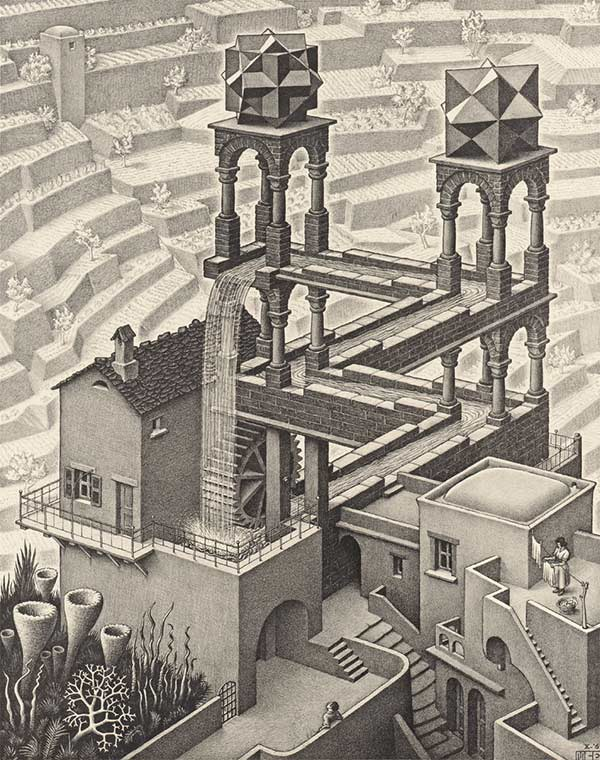
\includegraphics[scale=0.3]{img/Escher-Waterfall-1961.eps}
 \captionsetup{labelformat=empty}
 \caption{埃舍尔《瀑布》1961}
 \label{fig:Escher-Waterfall}
\end{wrapfigure}

1996年,第26界国际奥林匹克运动会正在美国的亚特兰大举行。来自世界各地的选手在速度、力量、技巧上展开竞赛挑战人类的极限。与此同时,还进行着另一场有趣的竞赛。超级计算机“深蓝”与人类的国际象棋世界冠军卡斯帕罗夫展开了对抗赛。比赛结果是深蓝2胜4负输给了人类象棋冠军。翌年,改进的深蓝再次向卡斯帕罗夫发起挑战。5月11日,计算机在正常时限的比赛中首次击败了卡斯帕罗夫。总比分1胜2负3平。深蓝计算机重1270公斤,有32个微处理器,每秒钟可以计算2亿步。为了能让"深蓝”挑战人类冠军,设计小组输入了一百多年来优秀棋手的对局两百多万对局。人类用智慧创造的机器,在人类骄傲的智慧领域首次击败了人类——这一结局引发了关注、恐惧、和激烈的讨论。

在当时,人们普遍认为,这是人工智能的一大进步。尽管在国际象棋上取得了巨大进步,但是在围棋上,计算机和人类仍存在巨大差距。对于国际象棋来说,棋盘8行8列,32枚棋子。计算机要在$10^{123}$这样巨大的博弈树中进行搜索。即使深蓝美妙能算2亿步,遍历博弈树仍需要近$10^{107}$年。为此深蓝的设计小组通过计算机程序缩小了搜索空间,使得深蓝能够搜索当前棋局后面的12步棋。而一般好的人类棋手,大约只能估计到10步左右。但是围棋的棋盘有19行19列,在一共361个格点上可以放置黑色或者白色的棋子。博弈树的规模为$10^{360}$,远远超越国际象棋。所以在之后的一段时间里,人们仍然不相信计算机可以挑战我们。

%\begin{wrapfigure}{R}{0.5\textwidth}
\begin{figure}[htbp]
 \centering
 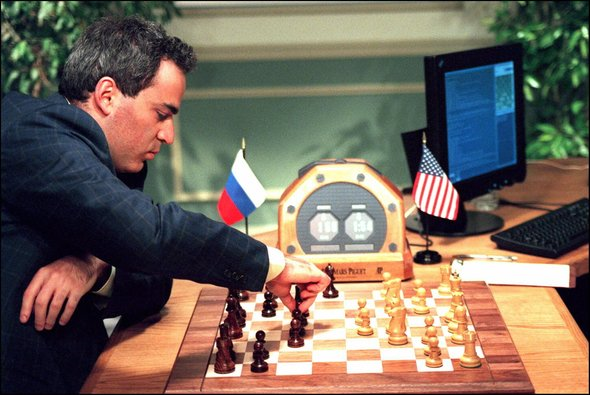
\includegraphics[scale=0.4]{img/Deep-blue-1997.eps}
 \captionsetup{labelformat=empty}
 \caption{卡斯帕罗夫在与深蓝对弈,图片原载《科学美国人杂志》}
 \label{fig:Deep-blue-1997}
\end{figure}
%\end{wrapfigure}

时光匆匆过去了20年,2016年,计算机程序Alpha-Go向人类的围棋大师展开了挑战。韩国的九段棋手李世石以1比4的总比分输掉了比赛。一年后,Alpha-Go再次以3局全胜的成绩战胜了中国棋手柯洁。被人们认为是人工智能游戏“圣杯”的围棋终于被攻破了。面对没有感情的计算机,柯洁心有不甘,潸然落泪。作为人类,我们的心情很复杂。即使是从事智力工作的程序员群体也感到了来自机器的压力——我们是否会被机器取代?

%University of Tubingen, Germany
% Leon A. Gatys, Alexander S. Ecker Matthias Bethge
传统上我们认为,艺术文学等领域,涉及人们的文化背景、内在感情和与生俱来的性格因素,是无法被机器所替代的。2015年,德国斯图加特以南40公里的小镇图宾根大学大学的盖提斯、埃克、贝特格三位研究人员利用机器学习人类艺术家的风格,把图宾根镇的一张风景照片变换成了不同风格的艺术画作\cite{Gatys-2015}。无论是后印象派大师梵高色彩强烈夸张的画风,还是透纳那浪漫主义水天浑浊的光影效果,都被机器模仿得惟妙惟肖。犹如大师本人所作(图\ref{fig:style-transfer})。

%\begin{wrapfigure}{R}{0.5\textwidth}
\begin{figure}[htbp]
 \centering
 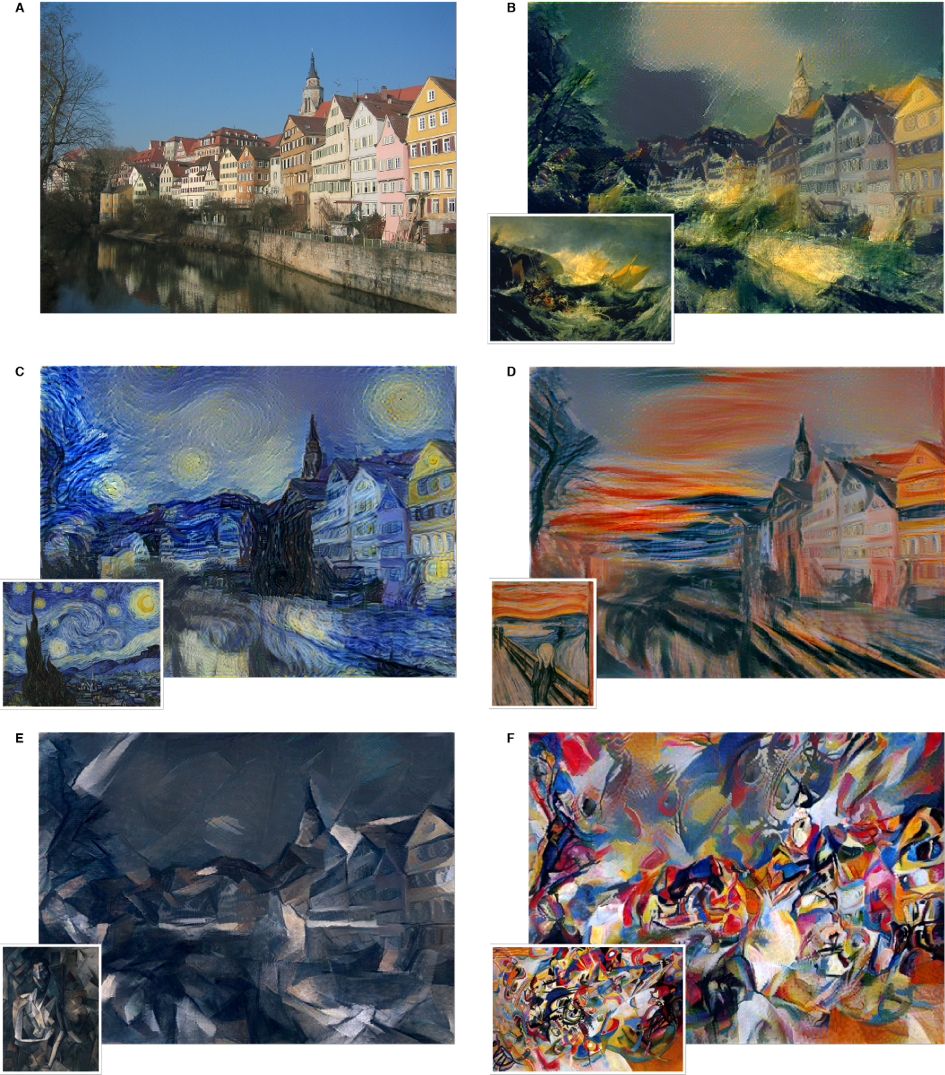
\includegraphics[scale=0.85]{img/style-transfer.eps}
 %\captionsetup{labelformat=empty}
 \caption{机器学习产生的不同艺术风格的画作:A,图宾根镇的风景照片;B,英国画家透纳1810年的原作《运输船遇难》和透纳风格的画作;C,荷兰后印象派画家梵高1889年的原作《星空》和梵高风格的画作;D,挪威表现主义画家爱德华$\cdot$蒙克1893年的原作《呐喊》和蒙克风格的画作;E,西班牙现代艺术家毕加索1910年的原作《坐着的裸女》和毕加索风格的画作;F,俄罗斯抽象艺术先驱画家康定斯基1913年的原作《构成第七号》和康定斯基风格的画作}
 \label{fig:style-transfer}
\end{figure}
%\end{wrapfigure}

在随后的数年中,人工智能和机器学习突飞猛进地进入了各种领域。机器产生不同音乐家风格的音乐,能够演奏出紧张、舒缓等不同的情绪的旋律和节奏,而不再是呆板单调的电子琴音。机器批量翻译新闻稿和各种学术论文,和专业翻译的文笔不相上下。机器处理X片、CT、核磁共振等医学图像并给出病理诊断,并且结果在准确程度上超越人类医生,人工智能操控的无人车在街道上行驶,成功超过其它车辆并避让行人。无人值守的商店突然出现在街边,人们可以直接从货架上拿走商品,并在走出商店的一刻自动支付……作为人类的我们不禁会问:我们消灭工作岗位的速度是否会超过创造工作机会的速度?人类是否会被机器全面取代?机器是否最终会统治我们?

所有这些在本质上都可以归结到一个问题:计算的能力是否存在边界?如果有的话,计算的边界在哪里?

\section{计算的边界}

顾森在《思考的乐趣》一书中讲到,注视着一个运行了很久的程序时的两难心情:这个程序能结束么?是应该继续等下去,还是杀掉进程强行结束?有没有什么编译器能事先告诉你的程序是否会无限运行下去?(\cite{GuSen-2012},第228页)

\begin{quotation}
为什么不可能呢?这个东西看上去比时光旅行机更现实一些。或许我们会在某个科幻电影中看到,一个程序员在漆黑的屏幕上输入几个数,敲了一下回车,然后屏幕上立即用高亮加粗字体显示:“警告:该输入数据会导致程序无限运行下去,确定执行?(Y/N)”如果有一天,这一切真的成为了现实。那么你能利用这个玩意儿来做些什么使用、有价值的事情?如果我说你能靠这玩意儿发大财的话,你相信么?……我上来就先写一个哥德巴赫猜想的验证程序。我写一个程序,让他从小到大枚举所有的偶数,看是不是有两个质数加起来等于它。如果找到来,继续枚举下一个偶数,否则输出反例并结束程序。然后编译该程序。这个编译器不是可以预先判断我这个程序能否终止吗?如果编译器说我这个程序会无限执行下去的话,我岂不是相当于证实来哥德巴赫猜想吗?或者,编译器说程序会最终终止,那哥德巴赫猜想不就直接被推翻来吗?不管怎样,我都将成为解决哥德巴赫猜想的第一人,在数学史上留下自己的名字。接下来呢?把刚才的程序代码改成孪生素数搜索器,在利用编译器检查一下,看看是不是真的有无穷多个孪生素数。梅森素数是否有无穷多个,这个也是数论中长期以来悬而未决的难题。不过现在看来,我也能不费吹灰之力就把它解决了。还记得$3x+1$问题吗?写一个“证明程序”也只是几分钟的事情,而且还能拿走埃尔德什提供的500美元奖金呢。数学上的未解之谜多着呢。我永远不愁没事做。1984年,马丁$\cdot$拉巴尔询问能否用9个不同的平方数构成$3 \times 3$幻方,这个问题的奖金目前已经积累到了100美元加100欧元再加一瓶香槟。网上搜索“数学未解难题”,看看哪些问题是离散的,其中又有哪些问题是有悬赏的,写几个程序就可以把它们统统解决……
\end{quotation}

1936年,计算机科学和人工智能的先驱图灵证明了一个命题:不存在可以判断任何程序是否可以停机的通用算法。证明的核心部分包含了计算机程序的数学定义——图灵机模型。后人称这一问题为图灵停机问题。

为了图灵证明停机问题,我们采用反证法,假设存在一个名叫$halts(p)$的算法,能够判断任意程序$p$是否停机。首先我们定义一个永不停机的程序:

\[
forever() = forever()
\]

这是一个无穷递归的调用。然后我们构造一个名为$G$的特殊程序\footnote{我们用字母$G$是有特殊用意的,$G$是哥德尔的首字母,它恰好和哥德尔不完全定理中不可判定命题的名字相同。},它的定义如下:

\[
G() = \begin{cases}
halts(G) = \text{停机}: & forever() \\
\text{否则}: & \text{停机} \\
\end{cases}
\]

在程序$G$中,我们通过$halts(G)$判断$G$本身是否停机。如果停机,我们就调用$forever()$永远运行下去。但这恰恰说明$G$不会停机,所以$halts(G)$应该为假,但是按照上面定义的第二行,此时我们停机。这恰恰说明$halts(G)$应该为真。所以不论$halts(G)$是真是假,我们都会得到矛盾的结论。因此我们最初的假设不成立,也就是说,不存在一个可以判断任意程序能否停机的通用算法。

也有一种分两步证明图灵停机问题的方法(\cite{SICP},第268页),前面都一样,但在构造$G$时,$G$接受一个参数$p$,它把$p$应用到自身上并传给$halts$:

\lstset{frame=single}
\begin{lstlisting}
G(p) = if halts(p(p)) then forever() else 'Halted'
\end{lstlisting}

接下来的一步中,我们把$G$传给自己$G(G)$看发生了什么?此时如果$halts(G(G))$返回真,则接下来运行$forever()$,所以$G(G)$永远运行不会停机。但这恰恰说明$halts(G(G))$应该返回假,所以接下来程序进入\texttt{else}分支,返回停机。但这又说明$halts(G(G))$应该返回真。所以不管停机与否,都陷入了矛盾之中。

伟大的图灵停机定理清晰地给出了一个不可计算问题。击碎了我们本节中给出的那些奇思妙想。看到这里,你是否想起了上一章附录中康托尔定理的证明?我们用极为类似的方法证明了任何集合,包括无穷集合的势都小于它的幂集的势。实际上,图灵停机问题让我们联想起了一大类有趣的逻辑悖论。

\section{罗素悖论}

% Eubulides of Miletus
悖论从古希腊时期就被人们发现了。上一章我们介绍了关于无穷和连续的芝诺悖论,而逻辑悖论是一类从严密逻辑导出矛盾结果的有趣问题。公元前四世纪,古希腊哲学家米利都的欧歩里德提出这样一个命题:“我现在说的是一句假话”,怎样判断这句话的真伪呢?

如果这句话是假话,那么它陈述的事实(正在说谎)就成了真的,因此矛盾。但如果这句话是真话,那么这句话的原话说正在说谎,因此它是假话,也产生了矛盾。不论欧歩里德说的是真是假,我们都将陷入矛盾中,这一著名的令人困惑的问题被人们称为“说谎者悖论”。

说谎者悖论还有一个两段体的变形,以对话的形式出现。例如:

\textbf{阿基里斯}:乌龟是个狡猾的家伙,总爱说谎,你听,它下面的话就是假的。

\textbf{乌龟}:亲爱的阿基里斯,诚实的你总是说真话。

乌龟的话到底是真是假呢?如果乌龟说了真话,也就是阿基里斯的陈述是真的。但阿基里斯说乌龟在撒谎,这就导致了矛盾。反之如果乌龟说的是假话,那么阿基里斯说的就是假的,于是乌龟说的这就话就应该为真。我们陷入了怪圈,无论乌龟的话是真是假,都会导致矛盾。

这种两段体式的说谎者悖论有时还以恶作剧的形式出现。你收到一张纸条,上面写着“背面是假的”,等你翻到纸条背面,却看到上面赫然写着“背面是真的”。到底哪面是真的呢?仔细分析下来,就会发现陷入了逻辑怪圈。

儿童故事中,也有不少这种悖论。有一则说狮子捉到了兔子,得意地说,如果你能猜中接下来我要干什么,我就放了你,要是猜错了,我就吃掉你。聪明的兔子说:“我猜你要吃掉我。”

如果狮子吃掉兔子,那说明兔子猜中了。这样狮子应该兑现承诺,放掉兔子。可是如果放掉兔子,这说明兔子猜错了。按道理狮子又应该吃掉兔子。狮子陷入了两难处境。既不能吃掉兔子,也不能不吃兔子。估计它只能发疯而让聪明的兔子溜走了。

传说古希腊的军队战胜了波斯,国王决心“优待俘虏”,让他们选择死亡的方式。俘虏可以说一句话,如果是真话,就被砍头,如果是假话,就被绞死。一个聪明的俘虏说:“我猜你要绞死我。”如果国王绞死了俘虏,说明他说了真话,可是这样,按照规则应该被砍头。但如果砍掉他的头,就和这个人讲的内容不符了,所以他说了假话。这样就应该被绞死。结果不论砍头还是绞死,国王的命令都没有被正确的执行。国王万般无奈,不仅释放了这个俘虏,还释放了所有其他人。

\begin{wrapfigure}{L}{0.5\textwidth}
 \centering
 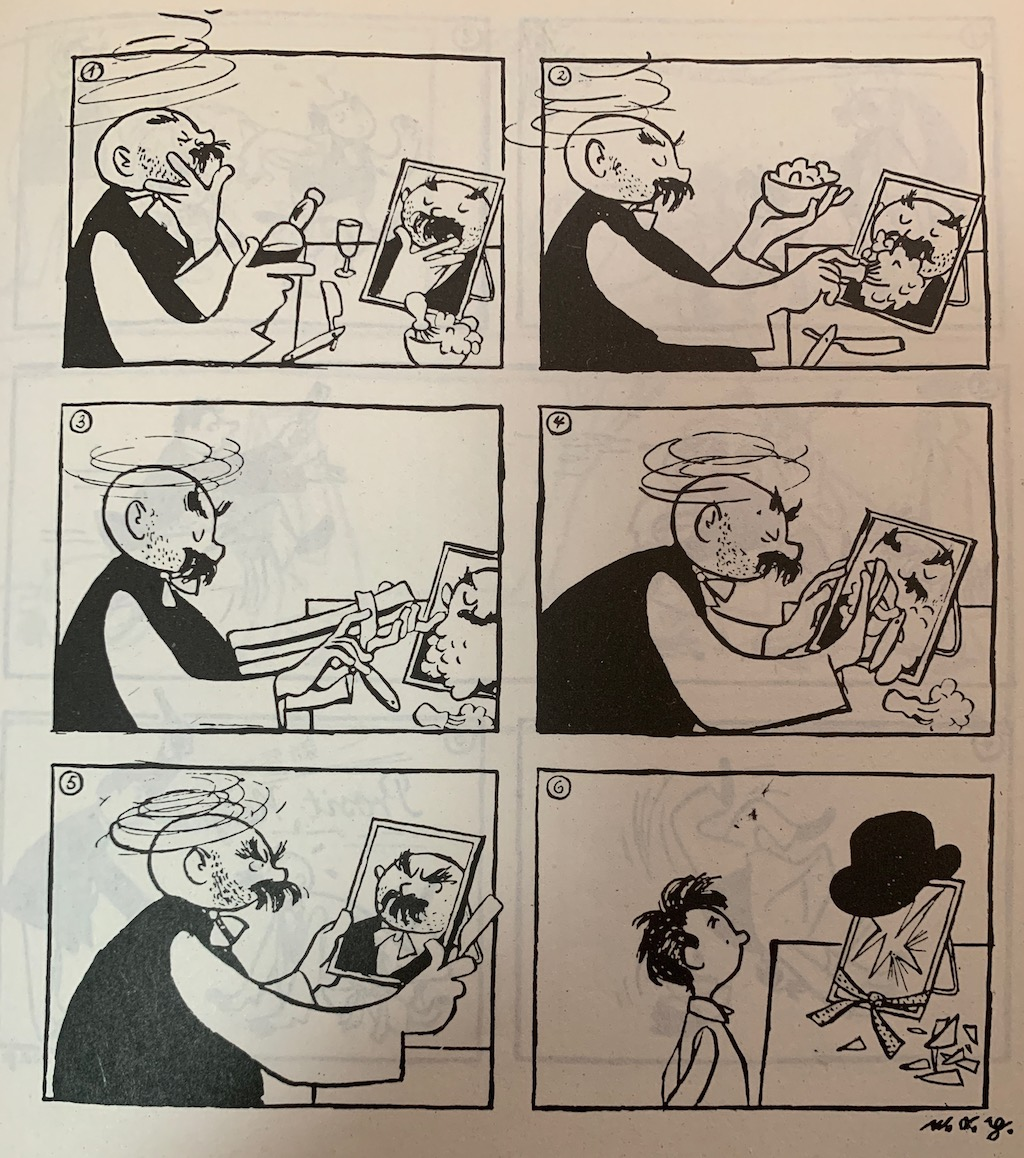
\includegraphics[scale=0.17]{img/father-and-son.eps}
 \captionsetup{labelformat=empty}
 \caption{[德]埃$\cdot$奥$\cdot$卜劳恩《父与子》一则,1930年代}
 \label{fig:father-and-son}
\end{wrapfigure}

塞万提斯在他的伟大作品《堂$\cdot$吉诃德》中,也讲了一个有趣的悖论。有一位贵族的封地被一条大河分成了两半,河上有一座桥,桥的尽头有个绞架。这位贵族制定了一条法令:“过桥的人必须诚实声明他的目的,如果是真话就允许过桥,如果说谎,就判处绞刑,绞死在桥那边的绞架上。”结果有个人来这里发誓道,我过桥别无目的,就是想死在那个绞架上。怎样处置这个人呢?如果他说了真话,那么就应该放他过桥。可是这样这个人说的内容就不成立了,按照法令就应该绞死他。可是这样以来他说的话就成了真话,又应该放他过桥。

% https://en.wikipedia.org/wiki/Barber_paradox
和说谎者悖论同样著名的是理发师悖论。这是1919年由著名数学家、逻辑学家罗素罗素提出的。故事说村子里的理发师宣布:“他只给那些不给自己刮胡子的人刮胡子。”那么这位理发师是否给他自己刮胡子?如果他给自己刮胡子,那么按照他的规定,他就不应该给自己刮胡子。而如果他不给自己刮胡子,那么他就应该向自己提供服务,也就是给自己刮胡子。理发师这样就会陷入了困境。

罗素归纳总结了一系列悖论,并最终将它们形式化为当时集合论本质上的问题。人们现在一般将这类悖论称为罗素悖论。罗素最早在1901年发现了集合论的悖论。在康托尔的朴素集合论中,罗素考虑了任何集合是否属于它自身的问题。有些集合属于它本身,有些集合则不属于。例如所有茶匙的集合显然不是另一个茶匙,但所有不是茶匙的东西构成的集合显然也不是一个茶匙。罗素考虑了后者这类情况全体构成的集合。他构造了集合$R$,由所有不是自身元素的集合所组成。用形式化的定义表示就是:

\[
R = \{ x | x \notin x \}
\]

罗素接着思考,$R$是否属于$R$呢?根据逻辑中的排中律,一个元素或者属于一个集合,或者不属于一个集合。因此对于一个给定的集合,问它是否属于自己是有意义的。但是这个定义良好的,看似合理的问题却陷入了两难境地。

如果$R$属于$R$,那么根据$R$的定义,它只包含不属于自身的元素构成的集合,应该有$R$不属于$R$。反之,如果$R$不属于$R$,同样根据定义,它包含不属于自身的集合,又应该有$R$属于$R$。不管属于或不属于,都会导致矛盾。形式化的表达就是:

\[
R \in R \iff R \notin R
\]

这样罗素就明确表明了康托尔的集合论中存在悖论。

\begin{wrapfigure}{R}{0.3\textwidth}
 \centering
 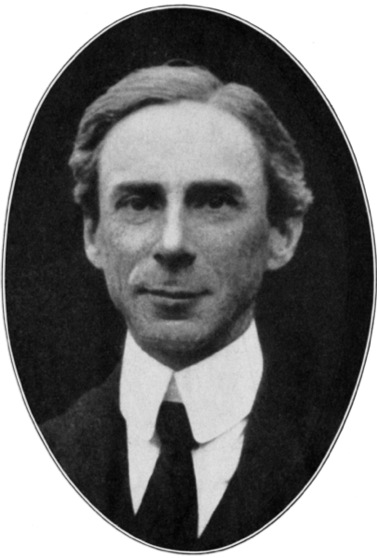
\includegraphics[scale=0.5]{img/Russell.eps}
 \captionsetup{labelformat=empty}
 \caption{伯特兰$\cdot$罗素 1872-1970}
 \label{fig:Russell}
\end{wrapfigure}

%Monmouthshire
罗素1872年生于英国蒙茅茨郡的一个贵族家庭。两岁时母亲去世,三岁时父亲也去世。6岁时祖父也去世了,于是罗素和祖母生活在一起。祖母对他的童年和青少年时期的发展有过决定性的影响。她曾告诫罗素:“你不应该追随众人去做坏事”,罗素一生都努力遵循这条准则。

罗素少年时代未被送到学校去学习,而是在家接受教育。1883年开始,11岁的罗素跟随堂哥弗兰克学欧几里德几何。不久,罗素开始接触哲学思辨,并在宗教问题上,悄悄写下自己的想法在一家杂志发表。1890年罗素考入剑桥大学三一学院,大学前三年,他专攻数学,获数学荣誉学位考试的第七名。1894年,参加伦理学荣誉学位考试。完成研究论文《论几何学的基础》。在剑桥期间,他结识了当时的数学讲师怀特海等人。1895年,罗素在三一学院获得了研究员的职位。二十世纪初,他发现了著名的罗素悖论,并引发了一场关于数学基础的大讨论。其后十多年间,罗素投身于数学基础和数理逻辑的研究中。1920年,罗素应邀到中国讲学一年。足迹遍及中华南北,作了多场演讲。话题从数理逻辑到切中时弊的社会改造建议,在当时成为中国文化界的一件盛事。给我国哲学界以很大的影响。他的《西方哲学史》在我国的哲学爱好者中有着广泛的影响。

二十世纪50年代后,罗素从哲学转向国际政治。他反对核战争、主张核裁军。由于伸张民主和参加核裁军运动,罗素一生曾两次被捕入狱。其中第二次入狱时已经是89岁高龄。1950年罗素获得诺贝尔文学奖。委员会在授奖时称他为“当代理性和人道的最杰出代言人之一,西方自由言论和自由思想的无谓斗士。”

1970年2月2日,罗素在彭林德拉耶斯逝世,他的骨灰被撒在威尔士的群山之中。
% Russell died of influenza on 2 February 1970 at his home in Penrhyndeudraeth. His body was cremated in Colwyn Bay on 5 February 1970. In accordance with his will, there was no religious ceremony; his ashes were scattered over the Welsh mountains later that year.

\subsection{罗素悖论的影响}

罗素发现集合论基础的悖论后极为沮丧。他后来回忆道:“每天早晨,我面对一张白纸坐在那儿,除了短暂的午餐,我一整天都盯着那张白纸。常常在夜幕降临之际,仍是一片空白……似乎我整个余生很可能就消耗在这张白纸上。让人更烦恼的是,矛盾是平凡的。我的时间都花在这些似乎不值得考虑的事情上。”(\cite{HanXueTao16},第231页)罗素把他的发现告诉了数学家、逻辑学家弗雷格。当时弗雷格正在进行算术基础的建立工作,他的著作《算术的基本规律》已在付印中。弗雷格看到罗素悖论后非常沮丧,他写道:“一个科学家所遇到的最不合心意的事莫过于在他工作即将结束时,其基础崩溃了。罗素先生的一封信正好把我置于这个境地。”戴徳金也推迟了《什么是数的本质》一书的再版。罗素悖论涉及的是集合论中最基础的部分。由于集合论逐渐被大家接受,并进入了大多数数学分支,这使得人们对于数学和逻辑学的基本原理和有效性产生了怀疑。

\begin{Exercise}
\Question{我们可以用语言定义数,例如“最大的两位数”定义了99。定义一个集合,是所有不能用20个以内的字描述的数字。考虑这样一个元素:“不能用20个以内的字描述的最小数”,它是否属于这个集合?}
\Question{“这个世界上唯一不变的是变化”——这句话是否是罗素悖论?}
\Question{本章开头苏格拉底的话是否是罗素悖论?}
\end{Exercise}

\section{数学基础的分歧}

逻辑主义

直觉主义

形式主义

\section{公理集合论}

\section{哥德尔不完全性定理}

\section{不完全性定理的证明}

\section{万能的程序与对角线证明}

\section{尾声}
理性思维的边界。

埃舍尔的龙
\begin{wrapfigure}{R}{0.5\textwidth}
%\begin{figure}[htbp]
 \centering
 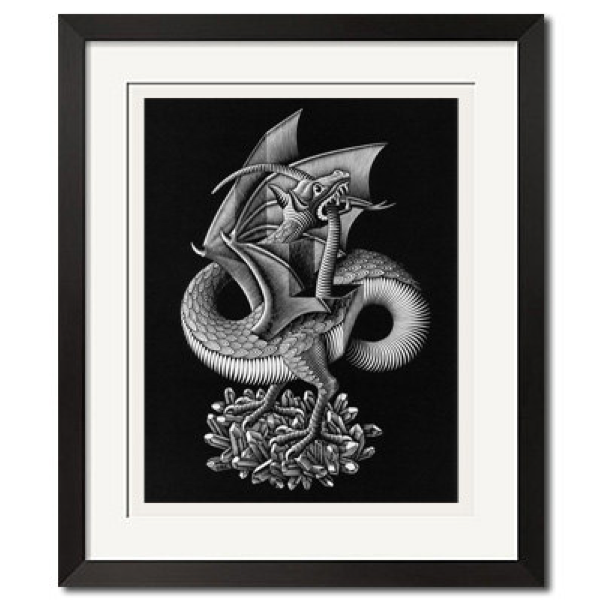
\includegraphics[scale=1]{img/Escher-Dragon.eps}
 %\captionsetup{labelformat=empty}
 \caption{埃舍尔《龙》}
 \label{fig:Escher-Dragon}
%\end{figure}
\end{wrapfigure}


\ifx\wholebook\relax \else
\begin{thebibliography}{99}

\bibitem{Gatys-2015}
Leon A. Gatys, Alexander S. Ecker, Matthias Bethge. ``A Neural Algorithm of Artistic Style.'' 2015. arXiv:1508.06576 [cs.CV] IEEE Conference on Computer Vision and Pattern Recognition (CVPR) 2017.

\bibitem{GuSen-2012}
顾森 《思考的乐趣——Matrix67数学笔记》 人民邮电出版社,2012年,ISBN: 9787115275868

\bibitem{SICP}
Harold Abelson, Gerald Jay Sussman, Julie Sussman 著 裘宗燕 译 ``计算机程序的构造和解释(原书第二版)''. 北京 机械工业出版社 2004年 ISBN: 7-111-13510-5

\bibitem{HanXueTao16}
韩雪涛 ``数学悖论与三次数学危机''. 人民邮电出版社. 2016, ISBN: 9787115430434

\end{thebibliography}

\expandafter\enddocument
%\end{document}

\fi
